
%(BEGIN_QUESTION)
% Copyright 2006, Tony R. Kuphaldt, released under the Creative Commons Attribution License (v 1.0)
% This means you may do almost anything with this work of mine, so long as you give me proper credit

A small-scale biodiesel manufacturing plant records the production of biodiesel fuel by measuring the liquid level in a storage vessel.  There is no flow transmitter monitoring flow rate into the vessel, but we can infer flow rate by monitoring vessel level over time.

$$\includegraphics[width=15.5cm]{i01504x02.eps}$$

The liquid level measurement signal coming from the ultrasonic level transmitter (LT) is our process variable (PV), and it is sent to a computer to be indicated and processed (LIU).  The particular processing done in the computer is calculation of average flow between sample intervals.

Suppose that the computer samples the transmitter's signal once every minute and records these measurements in a data file.  Here is an example of that file's contents after one tank-filling batch, shown in a table format:

% No blank lines allowed between lines of an \halign structure!
% I use comments (%) instead, so that TeX doesn't choke.

$$\vbox{\offinterlineskip
\halign{\strut
\vrule \quad\hfil # \ \hfil & 
\vrule \quad\hfil # \ \hfil & 
\vrule width2pt \quad\hfil # \ \hfil & 
\vrule \quad\hfil # \ \hfil & 
\vrule width2pt \quad\hfil # \ \hfil & 
\vrule \quad\hfil # \ \hfil \vrule \cr
\noalign{\hrule}
%
% First row
Time & Volume & Time & Volume & Time & Volume \cr
%
(minutes) & (gallons) & (minutes) & (gallons) & (minutes) & (gallons) \cr
%
\noalign{\hrule}
%
% Another row
0 & 17.05 & 10 & 31.12 & 20 & 40.15 \cr
%
\noalign{\hrule}
%
% Another row
1 & 17.05 & 11 & 33.89 & 21 & 42.22 \cr
%
\noalign{\hrule}
%
% Another row
2 & 17.05 & 12 & 36.69 & 22 & 44.60 \cr
%
\noalign{\hrule}
%
% Another row
3 & 17.05 & 13 & 39.40 & 23 & 47.16 \cr
%
\noalign{\hrule}
%
% Another row
4 & 17.05 & 14 & 40.15 & 24 & 50.00 \cr
%
\noalign{\hrule}
%
% Another row
5 & 17.05 & 15 & 40.15 & 25 & 52.85 \cr
%
\noalign{\hrule}
%
% Another row
6 & 20.06 & 16 & 40.15 & 26 & 55.76 \cr
%
\noalign{\hrule}
%
% Another row
7 & 23.01 & 17 & 40.15 & 27 & 58.64 \cr
%
\noalign{\hrule}
%
% Another row
8 & 25.44 & 18 & 40.15 & 28 & 61.53 \cr
%
\noalign{\hrule}
%
% Another row
9 & 28.23 & 19 & 40.15 & 29 & 64.31 \cr
%
\noalign{\hrule}
} % End of \halign 
}$$ % End of \vbox

\filbreak

Plotted over time on a graph, this data takes on the following form:

$$\includegraphics[width=15.5cm]{i01504x01.eps}$$

Just looking at this graph, what can you determine about the {\it flow rate} of biodiesel into this vessel?  What would account for the ``flat'' spot in the middle of the graph?  What do the minute variations in slope in the other areas of the graph represent, in terms of flow into the vessel?

\filbreak

Now, use the data in the table to calculate and plot the flow rate of biodiesel in gallons per minute into this vessel:

$$\includegraphics[width=15.5cm]{i01504x03.eps}$$

How do these two plots relate to each other?  That is, how does the {\it shape} of one refer to the {\it shape} of the other, geometrically?

\vskip 20pt \vbox{\hrule \hbox{\strut \vrule{} {\bf Suggestions for Socratic discussion} \vrule} \hrule}

\begin{itemize}
\item{} Suppose a technician decided to calculate the flow rate at $t =$ 4 minutes by taking the volume at that time (17.05 gallons) and dividing by the time (4 minutes).  Explain why this would yield an incorrect value for flow, then explain the correct way to calculate flow rate at that time from the given data.
\end{itemize}

\underbar{file i01504}
%(END_QUESTION)





%(BEGIN_ANSWER)

$$\includegraphics[width=15.5cm]{i01504x04.eps}$$

%(END_ANSWER)





%(BEGIN_NOTES)

The pattern should be clear: the {\it height} of the red (flow) plot at any point in time mirrors the {\it slope} of the blue (volume) plot.  This is to say, the flow plot is the {\it time-derivative} of the volume plot:

$$Q = {dV \over dt}$$

Closer to the truth, what we are actually calculating here is the {\it average} flow rate between time points, represented by the following equation:

$$Q = {\Delta V \over \Delta t}$$

%INDEX% Mathematics, calculus: derivative (calculating flow rates from measured volumes at specific times)
%INDEX% Process: biodiesel storage tank

%(END_NOTES)


